\chapter{Binäre Bäume}

\section{Lösung a}

\begin{itemize}
    \item Im \textbf{worst-case} liegen Einfügeoperationen in einem binären Suchbaum in der Komplexitätsklasse $O(n)$
    \item Im \textbf{average-case} liegen Einfügeoperationen in einem binären Suchbaum in der Komplexitätsklasse $O(log n)$
\end{itemize}

Im \textbf{}


\begin{figure}
    \begin{center}
        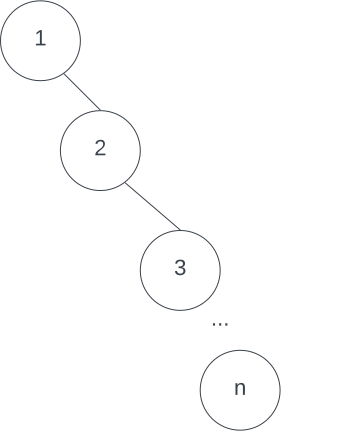
\includegraphics[scale=0.3]{chapters/5. Binäre Bäume/img/degenerate_tree}
        \caption{Für einen entarteten binären Suchbaum liegen Einfügeoperationen im \textbf{worst-case} in der Komplexitätsklasse $O(n)$ (Quelle: eigene)}
        \label{fig:degeneratetree}
    \end{center}
\end{figure}

\subsection{Anmerkung und Ergänzungen}


\noindent
In der Literatur wird manchmal die Definition \textbf{vollständiger} und \textbf{fast vollständiger} binärer Baum unterschiedlich gehandhabt.
Bei \textit{Ottmann und Widmayer} ist ein \textbf{vollständiger Baum} ein Baum, der auf jedem \textit{Niveau}\footnote{Knoten eines Baumes gleicher Tiefe} die maximal mögliche Knotenzahl hat und sämtliche Blätter dieselbe Tiefe haben (vgl.~\cite[261]{OW17e}).\\
Bei \textit{Güting und Dieker} entspricht die Definition der eines \textbf{fast vollständigen Baumes}, also ein Baum, der bis auf die letzte Ebene vollständig besetzt ist (vgl.~\cite[96]{GD18c}, außerdem~\cite[161]{CL22} und~\cite[401]{Knu97a}).\\
Wir folgen der Definition von \textit{Ottmann und Widmayer} (s. Skript (Teil 2), S.  101).\\

 \noindent
Der \textbf{worst-case} ergibt sich, wenn ein binärer Suchbaum \textbf{entartet}\footnote{
vgl. \cite[136]{GD18e}
} ist - die Reihenfolge der Knoten entspricht dann der Anordnung in einer verketteten List, in der das kleinste Element am Anfang der Liste steht, das größte Element am Ende der Liste.\\
Soll jetzt ein Element eingefügt werden, dessen Schlüssel größer als alle in dem Suchbaum enthaltenen Werte ist, muss der \textit{rechte Teilbaum} bis zum Ende durchwandert werden, um das Element einzufügen.\\
Bei $n$ vorhandenen Knoten ergibt sich somit ein Zeitaufwand von $O(n)$ (Nachweis u.a. bei~\cite[135 f.]{GD18d}).\\

\noindent
Für den \textbf{average-case} stellen \textit{Sedgewick und Wayne} fest:

\blockquote[{\cite[403]{SW11}}]{
The running time of algorithms on binary search trees depend on the shapes of the trees, which, in turn, depend on the order in which keys are inserted. In the best case, a tree with $N$ nodes could be perfectly balanced [...] the balance in typical trees turns out to be much closer to the best case than the worst case.
}\\

\noindent
Ein \textbf{balancierter Baum} ist ein Baum, bei dem die Differenz der Höhe des linken Teilbaums und die Höhe des rechten Teilbaums eines Knotens max. $1$ ist (vgl. \cite[284]{OW17e}).\\
Die maximale Pfadlänge in einem balancierten Baum ist $O(log\ n)$\footnote{$n=$ Anzahl der Knoten} (vgl.\cite[135]{GD18d}).\\
Hiermit ergibt sich im \textit{ungünstigsten Fall}, dass mindestens $O(log\ n)$ Operationen nötig sind, um einen Schlüssel für eine Einfügeoperation zu finden.\footnote{
In einem vollständigen Baum (\textit{nicht} Suchbaum!) mit $2^{h-1} - 1$ Knoten (mit $h$ = Höhe des Baumes) müssen im ungünstigsten Fall genausoviele (also der Anzahl der Knoten entsprechende) Vergleiche durchgeführt werden, um ein Blatt zu finden.
}\\
Eine vollständige Analyse, die für den \textbf{average-case} zu $O(log\ n)$ führt, findet sich bei \textit{Güting und Dieker} (~\cite[136 ff.]{GD18d}).




\section{Lösung b}

\begin{itemize}
    \item \textbf{Preorder}: $70,\ 50,\ 10,\ 25,\ 20,\ 45,\ 40,\ 35$
    \item \textbf{Inorder}: $10,\ 50,\ 20,\ 25,\ 70,\ 40,\ 35,\ 45$
    \item \textbf{Postorder}: $10,\ 20,\ 25,\ 50,\ 35,\ 40,\ 45,\ 70$
\end{itemize}


\subsection{Anmerkung und Ergänzungen}

Die eindeutige Rekonstruktion des Bäumes kann mithilfe der  \textbf{Preorder und Inorder}-Reihenfolge oder \textbf{Postorder und Inorder}-Reihenfolge realisiert werden.

\subsection*{Rekonstruktion mit Preorder \& Inorder}

\begin{enumerate}
    \item In der Preorder-Reihenfolge werden zuerst die Wurzelknoten besuche, dann der linke Teilbaum der Wurzel, dann der rechte (\textbf{KLR}).\\
    Knoten \textbf{(70)} kommt in der Preorder-Reihenfolge als erster Knoten vor, also muss das der Wurzelknoten des zu rekonstruierenden Baumes sein.\\
    Wir markieren \textbf{(70)} in der Inorder-Reihenfolge und kennen dadurch den linken und den rechten Teilbaum: Der linke Teilbaum muss die Knoten \textbf{(10, 50, 20, 25)} enthalten, der rechte Teilbaum die Knoten \textbf{(40, 35, 45)} (s. Abbildung~\ref{fig:reconstruction}).
    \item Im zweiten Schritt wird wieder zunächst die Reihenfolge der Knoten der Preorder-Reihenfolge untersucht: Der linke Teilbaum hat als einen Wurzelknoten die \textbf{(50)}, die wieder als Knoten in der Inorder-Reihenfolge markiert wird; gleiches passiert mit \textbf{(45)} des rechten Teilbaums der Preorder-Reihenfolge.\\
    Aus der Inorder-Reihenfolge lassen sich dann nach Markieren der Knoten weitere Teilbäume auslesen, die für den Knoten \textbf{(50)} den linken Teilbaum \textbf{(10)} und den rechten Teilbaum \textbf{(20, 25)} ergeben.
    Der Knoten \textbf{(45)} hat nur einen rechten Teilbaum mit dem Knoten \textbf{(40, 35)}.
    \item Im letzten Schritt werden die verbliebenen Teilbäume untersucht.\\
    Der Teilbaum in Prerorder-Reihenfolge \textbf{(25, 20)} und in Inorder-Reihenfolge \textbf{(20, 25)} kann zu dem eindeutigen Teilbaum \textbf{(20)} (linker Nachfolgerknoten) und \textbf{(25)} (Vorgängerknoten) rekonstruiert werden.\\
    Der Teilbaum \textbf{(40, 35)} in Preorder- und Inorder-Reihenfolge lässt sich zu dem eindeutigen Teilbaum \textbf{(40)} (Vorgängerknoten) und \textbf{(35)} (rechter Nachfolgerknoten) rekonstruieren.
\end{enumerate}

\begin{figure}
    \begin{center}
        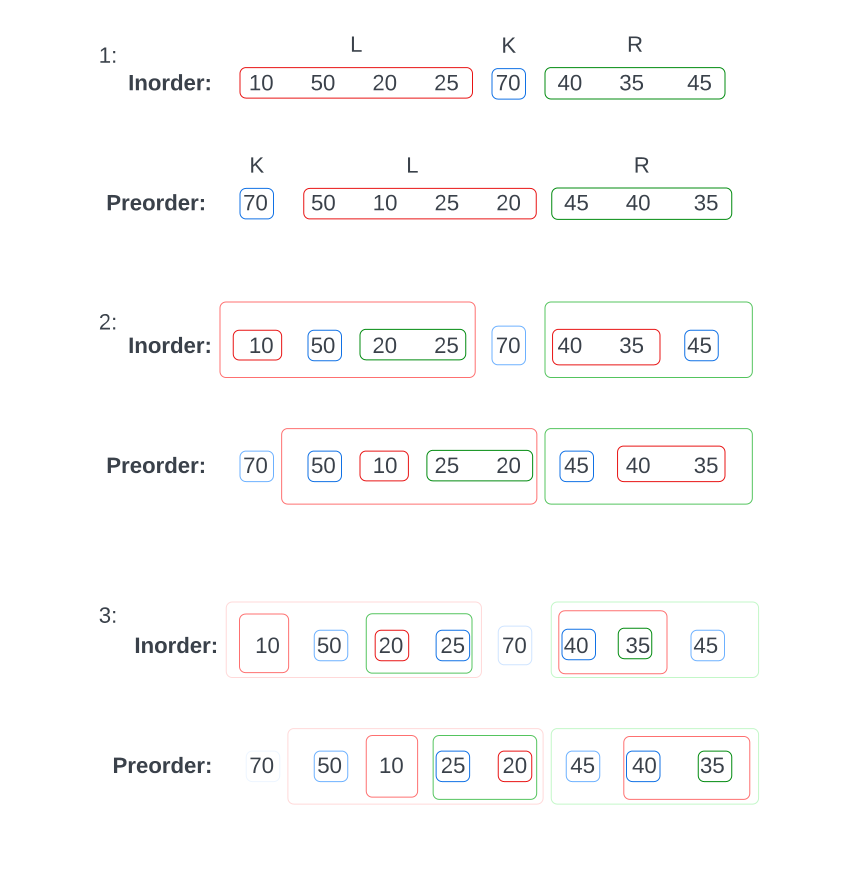
\includegraphics[scale=0.5]{chapters/5. Binäre Bäume/img/reconstruction}
        \caption{Rekonstruktion des Baumes anhand seiner Preorder- und Inorder-Reihenfolge (Quelle: eigene)}
        \label{fig:reconstruction}
    \end{center}
\end{figure}

Die Rekonstruktion anhand Postorder und Inorder erfolgt analog.

\newpage

\section{Lösung c}

Es gibt mehrere Bäume (s. Abbildung~\ref{fig:preproreconstruction}).


\begin{figure}
    \begin{center}
        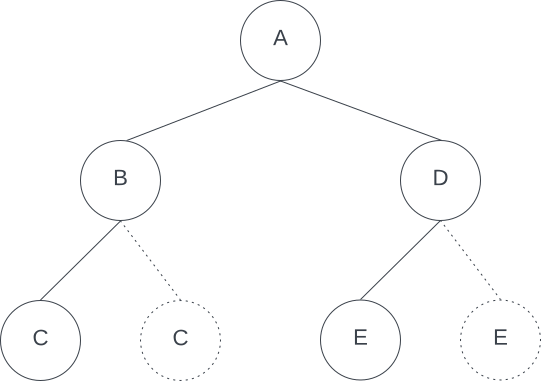
\includegraphics[scale=0.5]{chapters/5. Binäre Bäume/img/preproreconstruction}
        \caption{Die angegebenen Lienarisierungen werden von mehreren Bäumen gleichzeitig erfüllt (Quelle: eigene)}
        \label{fig:preproreconstruction}
    \end{center}
\end{figure}


\subsection{Anmerkung und Ergänzungen}

Die angegebenen Reihenfolgen $t_{Pre}$: A B C D E und $t_{Post}$: C B E D A lassen sich wie folgt untersuchen:

Der Baum $t_{Pre}$ hat als Wurzelknoten den Knoten \textbf{A}.\\
Der Baum $t_{Post}$ hat diesen Knoten ebenfalls als Knoten (s. Abbildung~\ref{fig:tree_a}).

\begin{figure}
    \begin{center}
        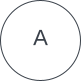
\includegraphics[scale=0.5]{chapters/5. Binäre Bäume/img/a}
        \caption{}
        \label{fig:tree_a}
    \end{center}
\end{figure}

\noindent
$t_{Pre}$: \textbf{A} B C D E\\
$t_{Post}$: C B E D \textbf{A}\\


\\
Es verbleiben die Teilbäume mit den Knoten \textbf{(B C D E)} (Preorder) sowie \textbf{(C B E D)} (Postorder).\\

\noindent
Für $t_{Pre}$ kann der Knoten \textbf{(B)} als linker Nachfolger von \textbf{(A)} verwendet werden.\\
Diese Bedingung kann auch von $t_{Post}$ erfüllt werden (s. Abbildung~\ref{fig:tree_ab}).

\begin{figure}
    \begin{center}
        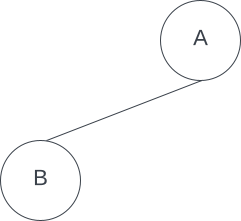
\includegraphics[scale=0.5]{chapters/5. Binäre Bäume/img/ab}
        \caption{}
        \label{fig:tree_ab}
    \end{center}
\end{figure}


Da \textbf{(C B E D)} in Postorder-Reihenfolge angegeben ist, muss folglich \textbf{(C)} ein Nachfolger von \textbf{(B)} sein, und zwar ein linker oder ein rechter Nachfolger. \\
Die Bedingung kann ebenfalls von $t_{Pre}$ erfüllt werden (s. Abbildung~\ref{fig:tree_abc}).\\

\begin{figure}
    \begin{center}
        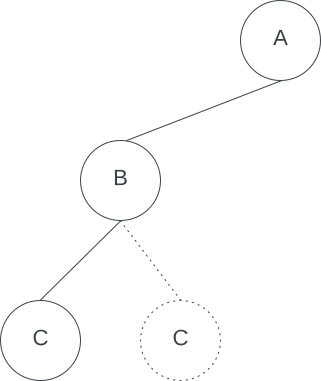
\includegraphics[scale=0.5]{chapters/5. Binäre Bäume/img/abc}
        \caption{}
        \label{fig:tree-abc}
    \end{center}
\end{figure}

\noindent
$t_{Pre}$: \textbf{A} \textbf{B C} D E\\
$t_{Post}$: \textbf{C B} E D \textbf{A}\\

\\
Mit \textbf{(B)} als direkter Nachfolger von dem Wurzelnoten \textbf{(A)} können jetzt aber \textbf{D} und \textbf{E} keine Vorgänger von \textbf{(B)} mehr sein für $t_{Post}$, sie sind somit Nachfolger von \textbf{A}.\\
Diese Bedingung läßt sich auch von $t_{Pre}$ erfüllen, \textbf{E} kann entweder linker oder rechter Nachfolger von $D$ sein (s. Abbildung~\ref{fig:tree_abcde}).\\


\begin{figure}
    \begin{center}
        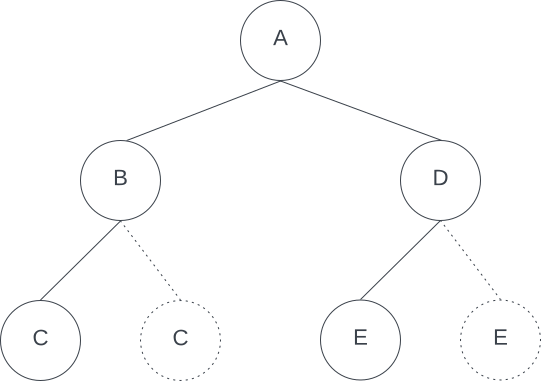
\includegraphics[scale=0.5]{chapters/5. Binäre Bäume/img/abcde}
        \caption{}
        \label{fig:tree_abcde}
    \end{center}
\end{figure}



